\section{Instrumenteringsforstærker}\label{sec:summa}
For at få en retning ud af spolesignalerne, anvendes instrumenteringsforstærkeren AD623. Instrumenteringsforstærkeren er valgt frem andre operationsforstærker typer, da den har meget større indgangsimpedans, hvilket er hensigtsmæssigt, da strømmene fra modtagerspolerne ikke er særligt store. Valget af instrumenteringsforstærkeren har også den fordel, at forstærkningen kan styres med blot en modstand, hvilket sparer plads på print boardet.

\begin{figure}[h!]
	\centering
	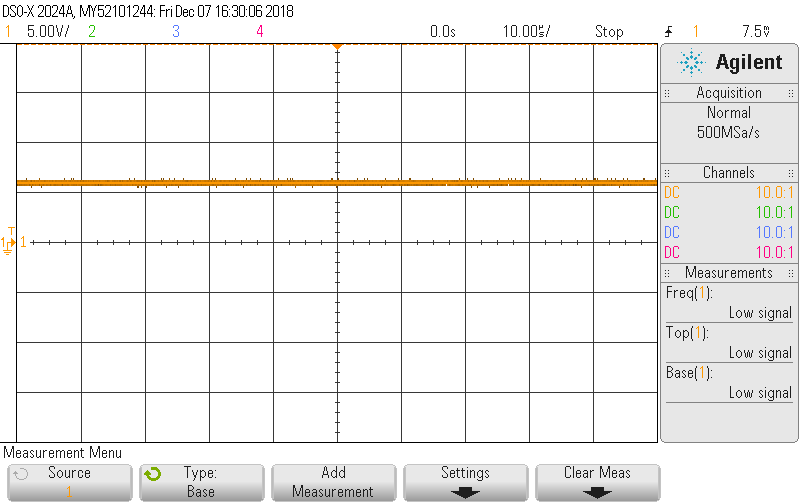
\includegraphics[width=1\textwidth]{billeder/instr_png.png}
	\caption{Billedet her viser outputtet fra instrumenteringsforstærkeren, hvor spolerne er i en tilfældig position.}
	\label{fig:filter_out}
\end{figure}

\subsection{Design}
Det samlede kredsløb for instrumenteringsforstærkeren består af en AD623, en gain modstand, samt et potentiometer. Dertil er der påsat to afkoblingskondensatorer. Kredsen forsynes med $\pm 7 \si{\volt}$, da det er max output fra batterierne. 

\husk{Kenneth}{Billede af instrumenterings kredsløb} 

\subsection{Beregninger}
\husk{Kenneth}{Find ud af spændingen før forstærkning. Også i filteret}
Da indgangssignalerne til instrumenteringsforstærkeren er meget lave, anvendes en gainmodstand for at forstærke signalet.

Der tilstræbes en forstærkning på 4 - 5 gange. Forstærkningen udregnes med ligning \ref{eq:GainModstand}.
\husk{Kenneth}{Link til datablad}
\begin{align}
	R_G & = \frac{100 \si{\kilo\ohm}}{G-1} \label{eq:GainModstand}
\end{align}
hvor en gainmodstand på 22 \si{\kilo\ohm} giver en forstærkning på 4.5.